\appendix
\section{Sample Tap Point Contents}


Here, we reproduce a selection of tap points from the same cluster as
dmesg and filename tap points.

\small

\begin{verbatim}
/etc/rc.d/ipfw/etc/rc.d/NETWORKING/etc/rc.d/netwait/etc/rc
.d/mountcritremote/etc/rc.d/devfs/etc/rc.d/ipmon/etc/rc.d/
mdconfig2/etc/rc.d/newsyslog
\end{verbatim}

\begin{verbatim}
r=/sNsnWs/fuiebu/ r=ceremdsecd_t_co_artpachg=tSooadSebaabf
/faa_N_=_peOfA=fA=feTr=tul.n=_eo/.b_Yt_vtectvifat=a=-sd_Ee
Ofu=u_0y:nF:tRseeeeEfciOtmdtuinlrlrrlpp/nppfpcepinl=l=.llN
lNlgllpl_.4l_l_2/l_l_22lileldlylo- 21laltlat=rrrsbgrskgni/
\end{verbatim}

\begin{verbatim}
russian|Russian Users Accounts:  :charset=KOI8-R:        :
lang=ru_RU.KOI8-R:     :       :passwd_format=md5:     :co
pyright=/etc/COPYRIGHT:      :welcome=/etc/motd:     :sete
nv=MAIL=/var/mail/$,BLOCKSIZE=K,FTP_PASSIVE_MODE=YES:     
\end{verbatim}

\begin{verbatim}
nss_compat.so.1dhclientShared object ``nss_compat.so.1'' n
ot found, required by ``dhclient''nss_nis.so.1dhclientShar
ed object ``nss_nis.so.1'' not found, required by ``dhclie
nt''nss_files.so.1dhclientShared object ``nss_files.so.1''
\end{verbatim}

\begin{verbatim}
digraph geom {
z0xc1d8de00 [shape=box,label=''PART\nada0\nr#2''];
z0xc1f4f640 [label=''r1w0e0''];
z0xc1f4f640 -> z0xc1e9eb00;
\end{verbatim}

\begin{verbatim}
/sbin/in/bin/sh/bin/stt/sbin/sysctl/bin/ps/sbin/sysctl/sbi
n/rcorde/bin/cat/sbin/md/sbin/sysctl/sbin/sysctl/bin/ken/s
bin/dumpon/bin/ln/bin/ps/sbin/sysctl/sbin/sysctl/sbin/sysc
tl/sbin/sysctl/bin/ps/bin/dd/sbin/sysctl/bin/dat/bin/df/sb
\end{verbatim}

\begin{verbatim}
/boot/kernel/kernel00000000-0000-0000-0000-000000000000000
00000-0000-0000-0000-00000000000000000000-0000-0000-0000-0
00000000000993c915d-3e9f-11e2-a557-525400123456993c915d-3e
9f-11e2-a557-525400123456/boot/kernel/kernel/boot/kernel/k
...
modulesoptions       CONFIG_AUTOGENERATED
ident   GENERIC
machine i386
cpu     I686_CPU
cpu     I586_CPU
cpu     I486_CPU
\end{verbatim}

\begin{verbatim}
<mesh>
  <class id=''0xc10362c0''>
    <name>FD</name>
  </class>
  <class id=''0xc1009a80''>
\end{verbatim}

\begin{verbatim}
#!/bin/sh
#
# $FreeBSD: release/9.0.0/etc/rc.d/newsyslog 197947 2009-1
0-10 22:17:03Z dougb $
...
set_rcvar()
{
        case $# in
        0)
                echo ${name}_enable
                ;;
        1)
\end{verbatim}


\begin{figure}[t]
    \begin{center}
        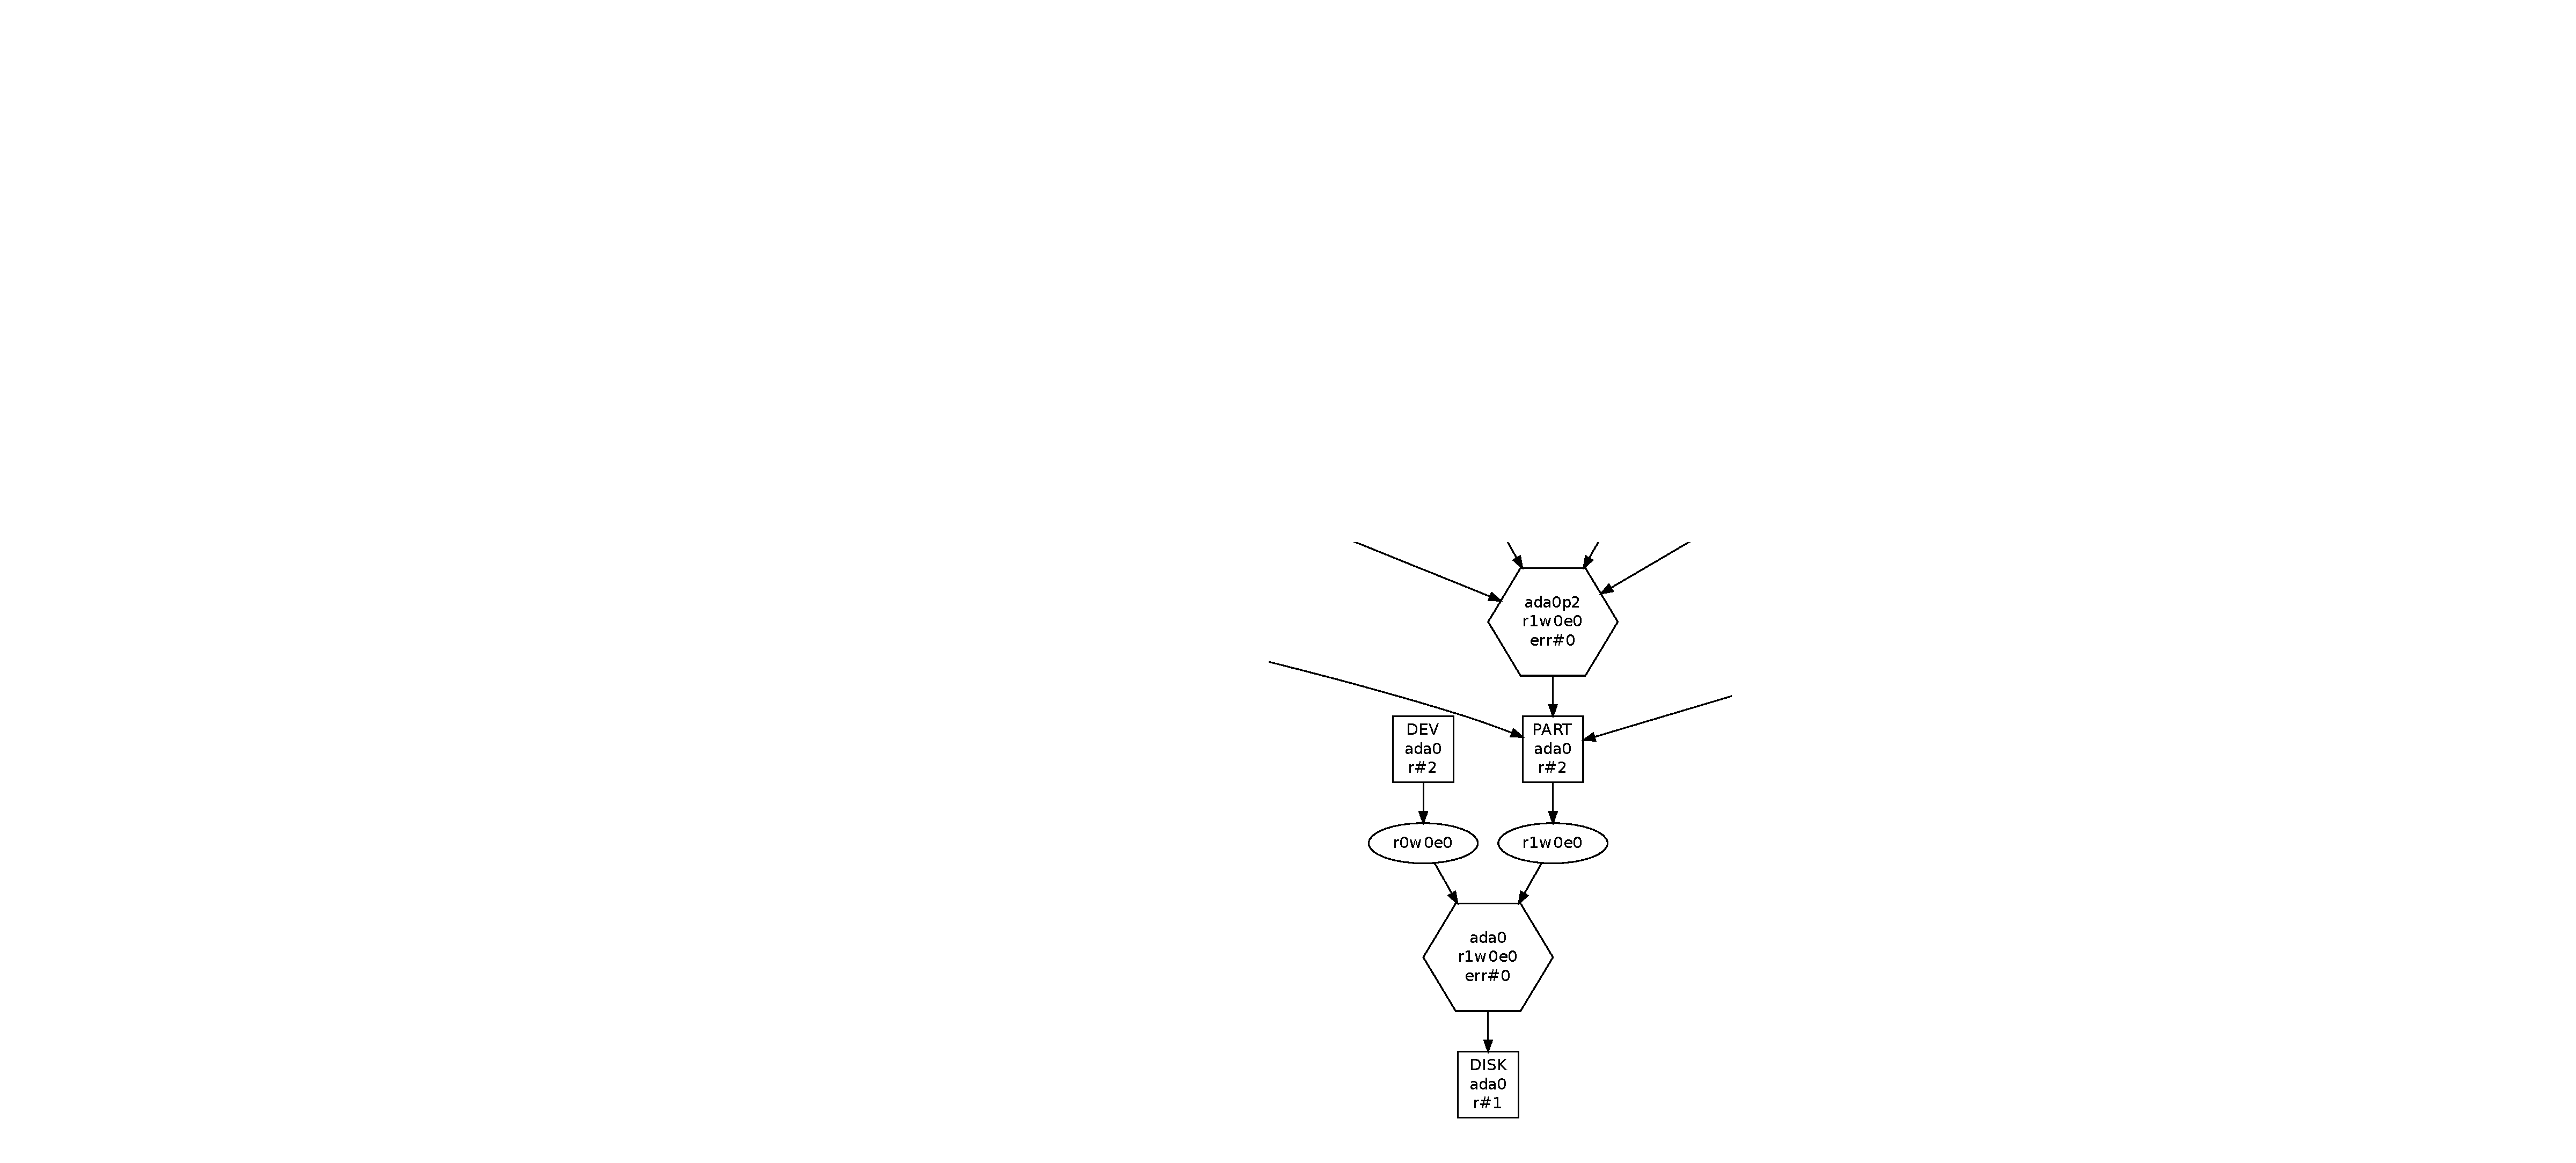
\includegraphics[width=2in]{figures/freebsd_graphviz.pdf}
    \end{center}
    \caption{Detail from rendering of Graphviz file captured from a FreeBSD
boot tap point, apparently depicting disk geometry}
    \label{fig:graphviz}
\end{figure}




